\documentclass[12pt]{standalone}

\RequirePackage{times}
\RequirePackage{amsmath}
\RequirePackage{amssymb}
\RequirePackage[T1]{fontenc}

\usepackage{tikz}
\usepackage{xcolor}
\usepackage{pgfplots}
\pgfplotsset{compat=1.16}

\definecolor{red}{HTML}{972e21}
\definecolor{yellow}{HTML}{ebb83f}
\definecolor{blue}{HTML}{7999db}

\begin{document}
	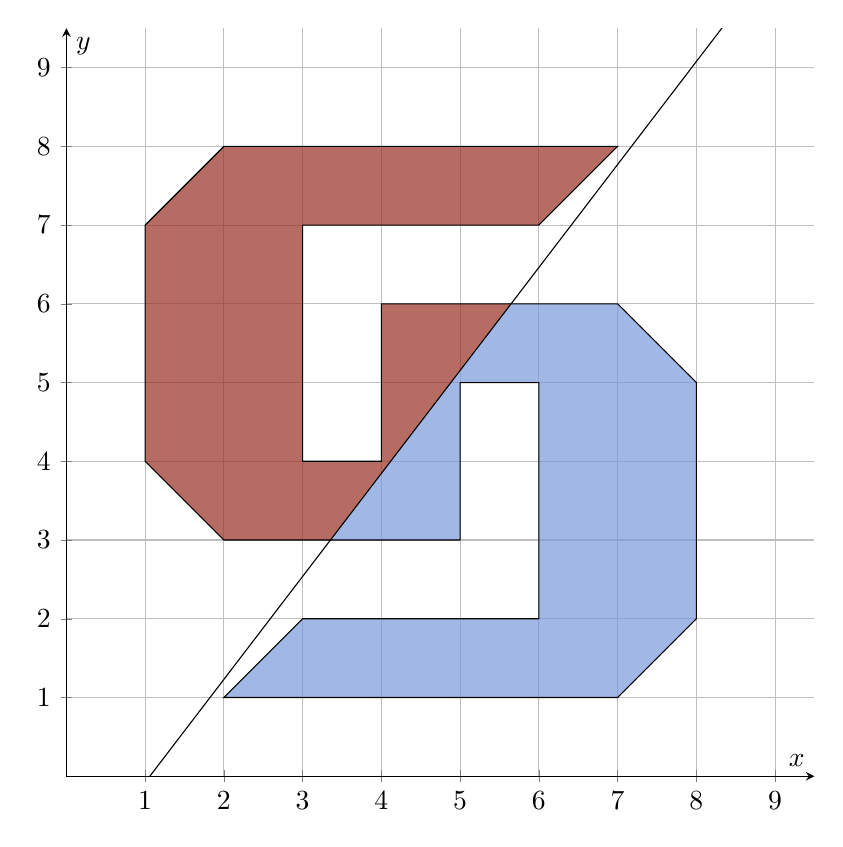
\begin{tikzpicture}
		\newcommand{\polygon}{
			(7, 1) --
			(8, 2) --
			(8, 5) --
			(7, 6) --
			(4, 6) --
			(4, 4) --
			(3, 4) --
			(3, 7) --
			(6, 7) --
			(7, 8) --
			(2, 8) --
			(1, 7) --
			(1, 4) --
			(2, 3) --
			(5, 3) --
			(5, 5) --
			(6, 5) --
			(6, 2) --
			(3, 2) --
			(2, 1) -- cycle}
		
		\begin{axis}[
			x=1.0cm,y=1.0cm,
			axis lines=middle,
			ymajorgrids=true,
			xmajorgrids=true,
			xmin=-0,
			xmax=9.5,
			ymin=-0,
			ymax=9.5,
			xtick={0.0,1.0,...,9.0},
			ytick={0.0,1.0,...,9.0},
			xlabel={$x$},
			ylabel={$y$},]
		
			% red
			\begin{scope}
				\clip \polygon;
				\fill[red,opacity=0.7] (11, 13) -- (-2,-4) -- (0,9) -- cycle;
			\end{scope}	
			
			% blue
			\begin{scope}
				\clip \polygon;
				\fill[blue,opacity=0.7] (11, 13) -- (-2,-4) -- (9,0) -- cycle;
			\end{scope}
			
			% cut
			\begin{scope}
				\clip (0,0) rectangle (9.5,9.5);
				\draw (11, 13) -- (-2,-4);
			\end{scope}
			
			% outline
			\draw \polygon;
		\end{axis}
	\end{tikzpicture}
\end{document}